\documentclass[tikz,border=8pt]{standalone}
% Shared look for every TikZ diagram. Load with \input{../../tools/tikz-style.tex}
\usepackage[T1]{fontenc}
\usepackage{lmodern}
\renewcommand{\sfdefault}{lmr}  % diagrams use the same serif as the text
\usetikzlibrary{arrows.meta, positioning, shapes.geometric, calc, fit, backgrounds}
\definecolor{cblue}{HTML}{4C78A8}
\definecolor{corange}{HTML}{F58518}
\definecolor{cgreen}{HTML}{54A24B}
\definecolor{cred}{HTML}{E45756}
\definecolor{cpurple}{HTML}{B279A2}
\definecolor{cgrey}{HTML}{6B6B6B}
\tikzset{
  every picture/.style={font=\sffamily, line width=1.2pt},
  box/.style={draw=#1, fill=#1!12, rounded corners=4pt, align=center, inner sep=7pt, minimum height=1.1cm},
  box/.default=cgrey,
  arrow/.style={-{Stealth[length=3mm]}, draw=cgrey, line width=1.4pt},
  title/.style={font=\sffamily\bfseries\Large},
  note/.style={font=\sffamily\small, text=cgrey, align=center},
}
\AtBeginDocument{\hyphenpenalty=10000 \exhyphenpenalty=10000}

\begin{document}
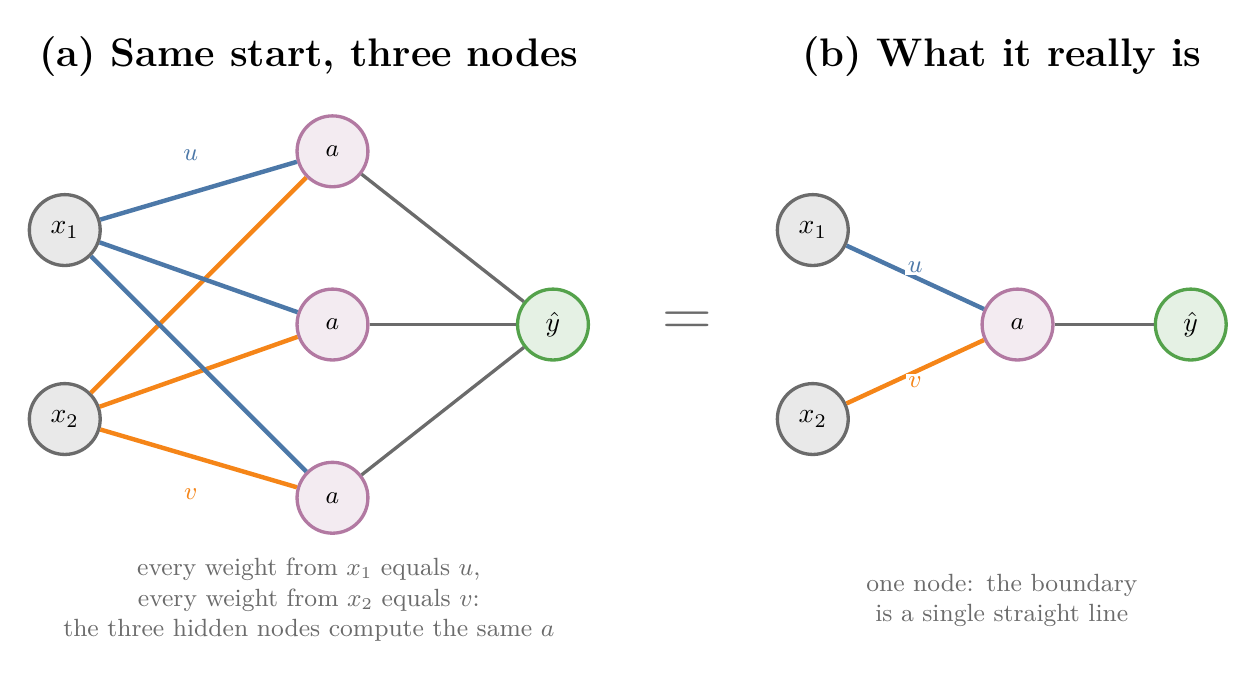
\begin{tikzpicture}[
  inp/.style={circle, draw=cgrey, fill=cgrey!15, minimum size=0.9cm, inner sep=0pt},
  hid/.style={circle, draw=cpurple, fill=cpurple!15, minimum size=0.9cm, inner sep=0pt, font=\sffamily\small},
  lab/.style={font=\sffamily\small, fill=white, inner sep=1pt}]
  % ---- (a) three tied nodes
  \node[inp] (x1) at (0,1.2) {$x_1$};
  \node[inp] (x2) at (0,-1.2) {$x_2$};
  \foreach \j/\yy in {1/2.2, 2/0, 3/-2.2} \node[hid] (h\j) at (3.4,\yy) {$a$};
  \node[circle, draw=cgreen, fill=cgreen!15, minimum size=0.9cm] (o) at (6.2,0) {$\hat{y}$};
  \foreach \j in {1,2,3} {
    \draw[cblue, line width=1.6pt] (x1) -- (h\j);
    \draw[corange, line width=1.6pt] (x2) -- (h\j);
    \draw[cgrey, line width=1.2pt] (h\j) -- (o);
  }
  \node[lab, text=cblue] at (1.6,2.15) {$u$};
  \node[lab, text=corange] at (1.6,-2.15) {$v$};
  \node[note, text width=6.5cm] at (3.1,-3.5) {every weight from $x_1$ equals $u$, every weight from $x_2$ equals $v$:\\the three hidden nodes compute the same $a$};
  \node[title] at (3.1,3.4) {(a) Same start, three nodes};
  % equals
  \node[font=\sffamily\Huge, text=cgrey] at (7.9,0) {$=$};
  % ---- (b) one node
  \begin{scope}[xshift=9.5cm]
    \node[inp] (y1) at (0,1.2) {$x_1$};
    \node[inp] (y2) at (0,-1.2) {$x_2$};
    \node[hid] (k) at (2.6,0) {$a$};
    \node[circle, draw=cgreen, fill=cgreen!15, minimum size=0.9cm] (p) at (4.8,0) {$\hat{y}$};
    \draw[cblue, line width=1.6pt] (y1) -- node[lab, above] {$u$} (k);
    \draw[corange, line width=1.6pt] (y2) -- node[lab, below] {$v$} (k);
    \draw[cgrey, line width=1.2pt] (k) -- (p);
    \node[note, text width=5cm] at (2.4,-3.5) {one node: the boundary\\is a single straight line};
    \node[title] at (2.4,3.4) {(b) What it really is};
  \end{scope}
\end{tikzpicture}
\end{document}
